\section{摩擦力}

\subsection{滑动摩擦力}
\subsubsection{相对运动时的摩擦力}

\begin{proset}
    如图所示，均匀\(T\)型物块\(A\)质量为\(m\)，夹在两个相同的水平垫板中，\(A\)与垫板间的动摩擦因数为\(\mu\)，垫板\(B\)、\(C\)以相同的水平速率\(v_1\)对称且匀速地向两侧退开，作用在\(A\)中央位置上的水平拉力\(F\)使\(A\)以速率\(v_2\)匀速前移，则下列说法正确的是\paren[A]

    \begin{tikzpicture}[font=\scriptsize,>=latex]
        \draw (.15,-.8)--++(60:1);
        \draw[fill=white] (-.7,.3)coordinate(a)--(.7,.3)coordinate(b)--(.7,0)coordinate(c)--(.15,0)--(.15,-.8)--(-.15,-.8)--(-.15,0)--(-.7,0)--cycle;
        \draw[fill=orange!40] (-1.4,0)coordinate(d) rectangle(-.3,-.2) (1.4,0)coordinate(e)  rectangle(.3,-.2);
        \draw[->,red] (0,-.1)--++(-120:.8)node[left]{\(F\)};
        \draw[->,blue] ($(0,.2)+(60:.8)$)node[above]{\(v_2\)}--++(-120:.6);
        \draw[->,blue] (-.5,-.1)--node[below]{\(v_1\)}(-1.2,-.1);
        \draw[->,blue] (.5,-.1)--node[below]{\(v_1\)}(1.2,-.1);
        \coordinate (f)at(1.4,-.2);
        \foreach \c in {a,b,c,d,e,f}
            \draw (\c)--++(60:1);
        \node[right] at(f){\(C\)};
        \node[left] at(-1.4,-.2){\(B\)};
        \node at(0,.1){\(A\)};
    \end{tikzpicture}
    \begin{choices}
        \item 增大匀速前移速率\(v_2\)，两侧垫板对\(A\)摩擦力的合力也增大
        \item 增大\(v_1\)，垫板\(B\)对\(A\)的摩擦力增大
        \item 恒力\(F\)的大小与\(v_1\)、\(v_2\)的大小无关
        \item 两侧垫板对\(A\)摩擦力的方向与水平向后的夹角\(\alpha\)均满足\(\tan\alpha = \frac{v_2}{v_1}\)
    \end{choices}
\end{proset}
\begin{answer}
    A\qquad 提示：\(A\)对\(B\)、\(C\)的正压力\(N = \frac{1}{2}mg\)大小不变，滑动摩擦力\(f =\mu N\)大小不变，方向与\(A\)相对\(B\)（或\(C\)）的速度\(u = v_2 - v_1\)方向相反，运动速度的俯视图如下：
    \begin{figure}[htbp]
        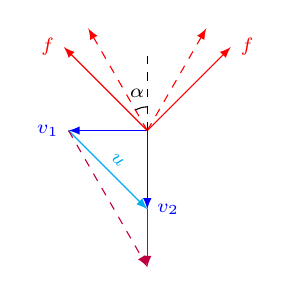
\begin{tikzpicture}[font=\scriptsize,>=latex]
        \draw[->,blue] (0,0)--(0,-1)node[right]{\(v_2\)};
        \draw[->,blue] (0,0)--(-1,0)node[left]{\(v_1\)};
        \draw[->,cyan] (-1,0)--node[above,rotate=-45]{\(u\)}(0,-1);
        \draw[->,red] (0,0)--++(135:1.5)node[left]{\(f\)};
        \draw[->,red] (0,0)--++(45:1.5)node[right]{\(f\)};
        \draw[->,purple] (0,-1)--(0,{-sqrt(3)});
        \draw[->,purple,dashed] (-1,0)--++(-60:2);
        \draw[->,red,dashed] (0,0)--++(60:1.5);
        \draw[->,red,dashed] (0,0)--++(120:1.5);
        \draw[dashed] (0,0)--++(0,1);
        \draw (0,.3)arc(90:120:.3);
        \node[above] at(-.13,.3){\(\alpha\)};
        \end{tikzpicture}
    \end{figure}
    摩擦力的合力\(f_{\text{合}} = 2f\cos\alpha = mg\cos\alpha
    \)
\end{answer}